\documentclass[]{template/RapportPole}

\usepackage{lipsum}
\usepackage{authblk}
\usepackage{graphicx}
%% pour les tables, cf https://github.com/rstudio/rmarkdown/issues/1384 et https://haozhu233.github.io/kableExtra/awesome_table_in_pdf.pdf
\usepackage{longtable}
\usepackage{booktabs}
\usepackage{makecell}

%% pour kable extra
%\usepackage{booktabs}
%\usepackage{longtable}
\usepackage{array}
\usepackage{multirow}
\usepackage{wrapfig}
\usepackage{float}
\usepackage{colortbl}
\usepackage{pdflscape}
\usepackage{tabu}
\usepackage{threeparttable}
\usepackage{threeparttablex}
\usepackage[normalem]{ulem}
\usepackage{makecell}
\usepackage{xcolor}

%% landscape mode
\usepackage{lscape}
\newcommand{\blandscape}{\begin{landscape}}
\newcommand{\elandscape}{\end{landscape}}

%% gestion des données de la page de titre
\title{Eel density analysis (EDA 2.3) : Modélisation de la biomasse des anguilles à l'échelle du territoire Français}
\subtitle{Rapport technique sur la préparation des données de pêches et la modélisation}
\reportType{2023}

% gestion des auteurs https://github.com/drdanholmes/Affiliations
%https://github.com/jolars/rmdplugr/blob/master/inst/latex-plugins/author-block.latex
% Author block
\IfFileExists{authblk.sty}{%
  \usepackage[]{authblk}
  \author[1,3]{Raitif Julien}
  \author[1,2,3]{BEAULATON Laurent}
  \author[3,4]{BRIAND Cédric}
  \author[1,3]{ANDRE Guirec}
  \affil[1]{OFB, Direction Recherche et appui scientifique, Service « Conservation et Gestion Durable des Espèces Exploitées »}
  \affil[2]{INRAE, Unité Expérimentale d'Ecologie et d'Ecotoxicologie aquatique}
  \affil[3]{\affilPole}
  \affil[4]{Etablissement Public Territorial de Bassin de la Vilaine}
}{
  \author{true}
  \author{true}
  \author{true}
  \author{true}
}

%% gestion du CSL pour pandoc >= 2.8
%description du pb https://github.com/rstudio/rmarkdown/issues/1649
%code repris de https://github.com/jgm/pandoc/blob/master/data/templates/default.latex


%% Autres
% gestion de l'erreur shaded https://stackoverflow.com/questions/41052687/rstudio-pdf-knit-fails-with-environment-shaded-undefined-error
\usepackage{color}
\usepackage{fancyvrb}
\newcommand{\VerbBar}{|}
\newcommand{\VERB}{\Verb[commandchars=\\\{\}]}
\DefineVerbatimEnvironment{Highlighting}{Verbatim}{commandchars=\\\{\}}
% Add ',fontsize=\small' for more characters per line
\usepackage{framed}
\definecolor{shadecolor}{RGB}{248,248,248}
\newenvironment{Shaded}{\begin{snugshade}}{\end{snugshade}}
\newcommand{\AlertTok}[1]{\textcolor[rgb]{0.94,0.16,0.16}{#1}}
\newcommand{\AnnotationTok}[1]{\textcolor[rgb]{0.56,0.35,0.01}{\textbf{\textit{#1}}}}
\newcommand{\AttributeTok}[1]{\textcolor[rgb]{0.13,0.29,0.53}{#1}}
\newcommand{\BaseNTok}[1]{\textcolor[rgb]{0.00,0.00,0.81}{#1}}
\newcommand{\BuiltInTok}[1]{#1}
\newcommand{\CharTok}[1]{\textcolor[rgb]{0.31,0.60,0.02}{#1}}
\newcommand{\CommentTok}[1]{\textcolor[rgb]{0.56,0.35,0.01}{\textit{#1}}}
\newcommand{\CommentVarTok}[1]{\textcolor[rgb]{0.56,0.35,0.01}{\textbf{\textit{#1}}}}
\newcommand{\ConstantTok}[1]{\textcolor[rgb]{0.56,0.35,0.01}{#1}}
\newcommand{\ControlFlowTok}[1]{\textcolor[rgb]{0.13,0.29,0.53}{\textbf{#1}}}
\newcommand{\DataTypeTok}[1]{\textcolor[rgb]{0.13,0.29,0.53}{#1}}
\newcommand{\DecValTok}[1]{\textcolor[rgb]{0.00,0.00,0.81}{#1}}
\newcommand{\DocumentationTok}[1]{\textcolor[rgb]{0.56,0.35,0.01}{\textbf{\textit{#1}}}}
\newcommand{\ErrorTok}[1]{\textcolor[rgb]{0.64,0.00,0.00}{\textbf{#1}}}
\newcommand{\ExtensionTok}[1]{#1}
\newcommand{\FloatTok}[1]{\textcolor[rgb]{0.00,0.00,0.81}{#1}}
\newcommand{\FunctionTok}[1]{\textcolor[rgb]{0.13,0.29,0.53}{\textbf{#1}}}
\newcommand{\ImportTok}[1]{#1}
\newcommand{\InformationTok}[1]{\textcolor[rgb]{0.56,0.35,0.01}{\textbf{\textit{#1}}}}
\newcommand{\KeywordTok}[1]{\textcolor[rgb]{0.13,0.29,0.53}{\textbf{#1}}}
\newcommand{\NormalTok}[1]{#1}
\newcommand{\OperatorTok}[1]{\textcolor[rgb]{0.81,0.36,0.00}{\textbf{#1}}}
\newcommand{\OtherTok}[1]{\textcolor[rgb]{0.56,0.35,0.01}{#1}}
\newcommand{\PreprocessorTok}[1]{\textcolor[rgb]{0.56,0.35,0.01}{\textit{#1}}}
\newcommand{\RegionMarkerTok}[1]{#1}
\newcommand{\SpecialCharTok}[1]{\textcolor[rgb]{0.81,0.36,0.00}{\textbf{#1}}}
\newcommand{\SpecialStringTok}[1]{\textcolor[rgb]{0.31,0.60,0.02}{#1}}
\newcommand{\StringTok}[1]{\textcolor[rgb]{0.31,0.60,0.02}{#1}}
\newcommand{\VariableTok}[1]{\textcolor[rgb]{0.00,0.00,0.00}{#1}}
\newcommand{\VerbatimStringTok}[1]{\textcolor[rgb]{0.31,0.60,0.02}{#1}}
\newcommand{\WarningTok}[1]{\textcolor[rgb]{0.56,0.35,0.01}{\textbf{\textit{#1}}}}

% gestion des listes avec les * (cf https://tex.stackexchange.com/questions/257418/error-tightlist-converting-md-file-into-pdf-using-pandoc)
\providecommand{\tightlist}{%
  \setlength{\leftskip}{3em}\setlength{\itemsep}{\leftskip}\setlength{\parskip}{0pt}}

\usepackage{hyperref} % nécessaire pour Rmd doit être mis en dernier (https://github.com/tabu-issues-for-future-maintainer/tabu/issues/24)
\hypersetup{
    colorlinks = true, % make the links colored
    linkcolor = black, % color TOC links in blue
    urlcolor = blue, % color URLs in red
    linktoc = all % 'all' will create links for everything in the TOC
}

\urlstyle{same}  % permet d'avoir la police des url identique au reste du texte

\begin{document}
%% Table des matières
{
\setcounter{tocdepth}{2}
\tableofcontents
}

\PageSuivanteStandard
\setcounter{page}{1}

%% Reste du documents
\hypertarget{introduction}{%
\chapter{Introduction}\label{introduction}}

Dans ce document, nous présenterons les différentes étapes qui sont réalisées afin de récupérer et préparer les données nécessaires.

\hypertarget{source-des-donnuxe9es}{%
\section{Source des données}\label{source-des-donnuxe9es}}

Le modèle EDA s'appuie aujourd'hui sur des données provenant de 2 sources différentes : - ASPE (Application de Saisie des données Piscicoles et Environnementales) - RSA (Réseau de Surveillance Anguilles)

\hypertarget{aspe}{%
\subsection{ASPE}\label{aspe}}

La base de données ASPE (Application de Saisie des données Piscicoles et Environnementales) est une base de données accessible en ligne (\url{https://aspe.eaufrance.fr/aspe-web/}).Elle permet aux personnes habilitées (personnel OFB essentiellement) de saisir les données techniques, environnementales,biologiques (effectifs capturés notamment) des opérations de pêches scientifiques. L'import de cette base peut se réaliser de deux façons :

\begin{itemize}
\tightlist
\item
  \textbf{Dump}
\end{itemize}

L'import des données ASPE se réalise grâce au fichier aspe\_import.R à partir d'un dump de la base de données ASPE fourni par XXXX. Ce dump est fourni ponctuellement (et à la demande) par XXXX. Cette version du rapportage anguille 2024 se base sur un dump en date du \texttt{25/06/2023}.

\begin{itemize}
\tightlist
\item
  \textbf{API Poisson}
\end{itemize}

Une autre technique d'accès aux données a été développée en se basant sur l'API Poisson (\url{https://hubeau.eaufrance.fr/page/api-poisson}) exploitée dans le fichier **test\_API\_JRT.R. Une requête est envoyée aux serveurs ASPE (maintenus par le BRGM) pour chaque année souhaitée. L'API est exploitée dans sa version paginée pour contourner la limitation de 20000 résultats par requête. Les résultats de la requête sont ainsi ``découpés'' en pages dont le nombre d'occurences est limité à 1000 pour optimiser les performances. Chaque page de résultats est ainsi parcouru et les occurrences sont compilées dans un dataset commun. L'avantage apportée par cette solution est l'autonomie d'accès aux données. L'inconvénient majeur et bloquant est qu'une grande partie des données nécessaire à l'exécution du modèle EDA (taille des stations notamment) est indisponible. Une version ultérieure (livraison fin 2023) pourrait potentiellement corriger cette limitation. Cette solution est donc abandonnée pour la mise à jour du rapport anguille 2024.

\hypertarget{rsa}{%
\subsection{RSA}\label{rsa}}

La base de données RSA est complémentaire de la base de données ASPE et accessible à un plus grand nombre d'utilisateurs, notamment les associations de pêches et autres partenaires des réseaux de surveillance des amphihalins. L'accès à ces données se fait par un dump de la base fourni par XXXX.

Cette version du rapportage anguille 2024 se base sur un dump en date du \texttt{07/07/2023}.

\hypertarget{pruxe9paration-des-donnuxe9es}{%
\chapter{Préparation des données}\label{pruxe9paration-des-donnuxe9es}}

A cette étape, et quelle que soit la source de données, l'objectif est de s'assurer de l'intégrité des données.

\hypertarget{aspe-1}{%
\section{ASPE}\label{aspe-1}}

La base de données ASPE contient un ensemble de données détaillant les opérations de pêches, les stations, les espèces pêchées. Toutes ces informations ne sont pas nécessaires pour EDA.

L'ensemble des étapes de préparations sont effectués dans le fichier \textbf{aspe\_import.R}.

\hypertarget{connexion-uxe0-la-base-eda-et-import-des-donnuxe9es-brutes}{%
\subsection{Connexion à la base EDA et import des données brutes}\label{connexion-uxe0-la-base-eda-et-import-des-donnuxe9es-brutes}}

Après chargement des librairies R, la connexion à la base de données EDA (sur laquelle se base le modèle) est initialisée. Les paramètres de connexion sont initialisées grâce au fichier \textbf{common/init.r}. A cette étape, les différents identifiants de connexion sont chargées depuis le fichier \textbf{EDAload23.xml} (cas où \texttt{rivernetwork==\ "RIOS"}). Dans le cas de l'import de données ASPE vers la base EDA, les paramètres de connexion utilisés sont repérés par les balises \textbf{lienODBCrios, uidrios et pwdrios}.

\begin{Shaded}
\begin{Highlighting}[]
\FunctionTok{options}\NormalTok{(}\StringTok{"width"}\NormalTok{)}

\NormalTok{con }\OtherTok{=} \FunctionTok{dbConnect}\NormalTok{(}\FunctionTok{Postgres}\NormalTok{(),}
        \AttributeTok{dbname=}\NormalTok{baseODBCrios[}\DecValTok{1}\NormalTok{],}
        \AttributeTok{host=}\StringTok{"localhost"}\NormalTok{,}
        \AttributeTok{port=}\DecValTok{5432}\NormalTok{,}
        \AttributeTok{user=}\NormalTok{baseODBCrios[}\DecValTok{2}\NormalTok{], }
        \AttributeTok{password=}\NormalTok{baseODBCrios[}\DecValTok{3}\NormalTok{])}
\end{Highlighting}
\end{Shaded}

Les données brutes issues du dump en date du 25/06/2023 sont ensuite chargées.

\begin{Shaded}
\begin{Highlighting}[]
\CommentTok{\# all data except biometry}
\FunctionTok{load}\NormalTok{(}\FunctionTok{str\_c}\NormalTok{(}\StringTok{"data/tables\_sauf\_mei\_2023\_06\_25\_21\_31\_13.RData"}\NormalTok{)) }
\CommentTok{\# biometry}
\FunctionTok{load}\NormalTok{(}\FunctionTok{str\_c}\NormalTok{(}\StringTok{"data/mei\_2023\_06\_25\_21\_31\_13.RData"}\NormalTok{))}
\end{Highlighting}
\end{Shaded}

\newpage

\hypertarget{filtre-sur-les-stations-en-france-muxe9tropolitaine}{%
\subsection{Filtre sur les stations en France métropolitaine}\label{filtre-sur-les-stations-en-france-muxe9tropolitaine}}

A cette étape du processus, un ensemble d'opérations de pêches sont présentes dans les différentes tables ASPE mais certaines concernent des stations se situant dans des pays frontaliers (Suisse, Allemagne, \ldots). Il convient de ne conserver que les stations françaises.

La première étape va être de charger toutes les stations présentes dans la table station et de ne conserver que celles dont la position est codifiée sur le système de coordonnées \textbf{Lambert-93\_France (code EPSG 2154)} puis de transformer ces coordonnées sur un référentiel européen \textbf{LAEA Europe (code EPSG 3035)}.

\begin{Shaded}
\begin{Highlighting}[]
\NormalTok{station\_aspe }\OtherTok{\textless{}{-}}\NormalTok{ station }\SpecialCharTok{\%\textgreater{}\%}
        \FunctionTok{left\_join}\NormalTok{(}\AttributeTok{y =}\NormalTok{ ref\_type\_projection, }
                  \AttributeTok{by =} \FunctionTok{c}\NormalTok{(}\StringTok{"sta\_typ\_id"} \OtherTok{=} \StringTok{"typ\_id"}\NormalTok{)) }\SpecialCharTok{\%\textgreater{}\%}
    \CommentTok{\# filter data from metropolitan France only }
    \CommentTok{\# (no overseas french territories). }
        \FunctionTok{filter}\NormalTok{(typ\_code\_epsg}\SpecialCharTok{==}\DecValTok{2154}\NormalTok{) }\SpecialCharTok{\%\textgreater{}\%}  
    \CommentTok{\#Spatial join will be performed }
    \CommentTok{\# to filter wrong coordinates later on}
        \FunctionTok{filter}\NormalTok{(sta\_coordonnees\_x }\SpecialCharTok{\textgreater{}} \DecValTok{0}\NormalTok{)}

\CommentTok{\# reproject coordinates in European system}
\CommentTok{\# from 2154\_Lambert{-}93\_France to 3035\_LAEA Europe}
\NormalTok{coords }\OtherTok{\textless{}{-}}\NormalTok{ aspe}\SpecialCharTok{::}\FunctionTok{geo\_convertir\_coords\_df}\NormalTok{(}\AttributeTok{df =}\NormalTok{ station\_aspe,}
        \AttributeTok{var\_x =}\NormalTok{ sta\_coordonnees\_x,}
        \AttributeTok{var\_y =}\NormalTok{ sta\_coordonnees\_y,}
        \AttributeTok{var\_id =} \StringTok{"sta\_id"}\NormalTok{,}
        \AttributeTok{var\_crs\_initial =} \StringTok{"typ\_code\_epsg"}\NormalTok{,}
        \AttributeTok{crs\_sortie =} \DecValTok{3035}\NormalTok{) }

\CommentTok{\# add reprojected coordinates to station\_aspe table}
\NormalTok{station\_aspe }\OtherTok{\textless{}{-}}\NormalTok{ station\_aspe }\SpecialCharTok{\%\textgreater{}\%}
        \FunctionTok{left\_join}\NormalTok{(}\AttributeTok{y =}\NormalTok{ coords) }\SpecialCharTok{\%\textgreater{}\%} 
    \CommentTok{\# dplyr::select({-}(sta\_geometrie)) \%\textgreater{}\%}
    \CommentTok{\#discard unused column}
\NormalTok{        dplyr}\SpecialCharTok{::}\FunctionTok{select}\NormalTok{(}\SpecialCharTok{{-}}\NormalTok{(sta\_geometrie),}\SpecialCharTok{{-}}\NormalTok{(}\FunctionTok{starts\_with}\NormalTok{(}\StringTok{"typ"}\NormalTok{))) }\SpecialCharTok{\%\textgreater{}\%} 
        \FunctionTok{mutate}\NormalTok{(}\AttributeTok{typ\_code\_epsg=}\DecValTok{3035}\NormalTok{) }

\CommentTok{\# remove all column starting with "typ"}
\NormalTok{station\_aspe }\OtherTok{\textless{}{-}}\NormalTok{ station\_aspe[,  }\SpecialCharTok{!}\FunctionTok{grepl}\NormalTok{(}\StringTok{"typ"}\NormalTok{,}\FunctionTok{colnames}\NormalTok{(station\_aspe))] }
\end{Highlighting}
\end{Shaded}

La liste de données \textbf{station\_aspe} est ensuite transformée en objet de type \textbf{spatial vector data (sf)} afin de pouvoir effectuer des opérations de manipulation cartographique. Nous allons notamment utiliser un un polygone ``France'' récupéré grâce au package R \textbf{rnaturalearth} qui sera croisé (intersection carto) avec l'objet sf des stations ASPE.

\newpage

Une précédente version de cette intersection provoquait la suppression de plus de 1000 stations (sur 33000 environ). Après investigation, ce filtre trop important provenait d'un polygone France trop grossier, notamment près des frontières (cf \textcolor{red}{points rouges} sur la figure ci-dessous).

\begin{Shaded}
\begin{Highlighting}[]
\NormalTok{station\_aspe\_sf }\OtherTok{\textless{}{-}} \FunctionTok{st\_as\_sf}\NormalTok{(station\_aspe, }\AttributeTok{coords=}\FunctionTok{c}\NormalTok{(}\StringTok{"X"}\NormalTok{,}\StringTok{"Y"}\NormalTok{),}\AttributeTok{crs=}\DecValTok{3035}\NormalTok{) }

\CommentTok{\# Spatial filtering}
\CommentTok{\#Get France polygons, projected in 3035\_LAEA Europe}
\NormalTok{france\_polygone }\OtherTok{\textless{}{-}}\NormalTok{ rnaturalearth}\SpecialCharTok{::}\FunctionTok{ne\_countries}\NormalTok{(}\AttributeTok{type =} \StringTok{"countries"}\NormalTok{, }
                \AttributeTok{country =} \StringTok{"france"}\NormalTok{, }
                \AttributeTok{returnclass =} \StringTok{"sf"}\NormalTok{) }\SpecialCharTok{\%\textgreater{}\%} 
  \CommentTok{\# keeps only name of country(\textquotesingle{}France") and its geometry}
        \FunctionTok{select}\NormalTok{(name\_sort) }\SpecialCharTok{\%\textgreater{}\%} 
  \CommentTok{\# reproject in the same crs as stations}
        \FunctionTok{st\_transform}\NormalTok{(}\DecValTok{3035}\NormalTok{) }

\CommentTok{\#to insure that all coordinate are correcly within France territory}
\CommentTok{\#intersect of stations dataset with france polygons}
\NormalTok{station\_aspe\_france }\OtherTok{\textless{}{-}}\NormalTok{ sf}\SpecialCharTok{::}\FunctionTok{st\_intersection}\NormalTok{( }
    \CommentTok{\# filter stations in France         }
\NormalTok{  station\_aspe\_sf, france\_polygone) }\SpecialCharTok{\%\textgreater{}\%} 
  \CommentTok{\# remove extra column from france polygone 31734}
    \FunctionTok{select}\NormalTok{(}\SpecialCharTok{{-}}\NormalTok{name\_sort) }
\CommentTok{\#deleted stations}
\NormalTok{station\_aspe\_france\_diff }\OtherTok{\textless{}{-}}\NormalTok{ sf}\SpecialCharTok{::}\FunctionTok{st\_difference}\NormalTok{(}
\NormalTok{  station\_aspe\_sf, france\_polygone)}
\CommentTok{\#visualisation }
\NormalTok{mapview}\SpecialCharTok{::}\FunctionTok{mapview}\NormalTok{(france\_polygone, }
                 \AttributeTok{alpha.regions =} \FloatTok{0.2}\NormalTok{, }
                 \AttributeTok{aplha =} \DecValTok{1}\NormalTok{,}\AttributeTok{legend=}\ConstantTok{FALSE}\NormalTok{) }\SpecialCharTok{+}
\NormalTok{  mapview}\SpecialCharTok{::}\FunctionTok{mapview}\NormalTok{(station\_aspe\_france\_diff, }
                   \AttributeTok{color=}\StringTok{"red"}\NormalTok{,}\AttributeTok{alpha.regions =} \FloatTok{0.1}\NormalTok{, }
                   \AttributeTok{aplha =} \FloatTok{0.1}\NormalTok{,}\AttributeTok{legend=}\ConstantTok{FALSE}\NormalTok{,}\AttributeTok{cex =}\DecValTok{1}\NormalTok{)}
\end{Highlighting}
\end{Shaded}

\begin{figure}
\centering
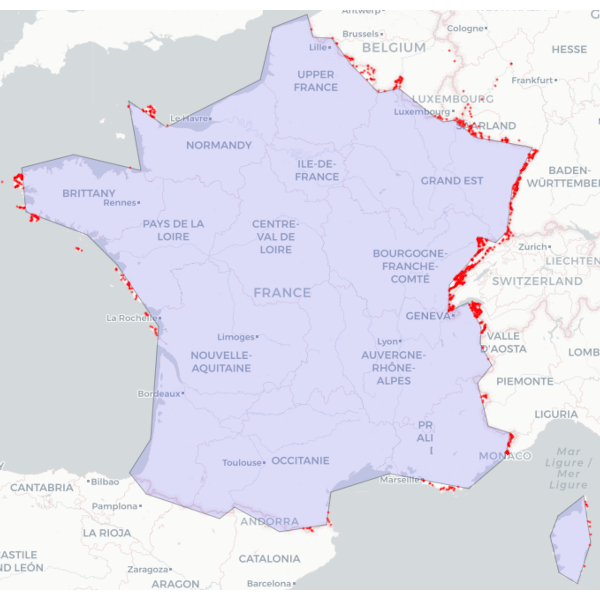
\includegraphics{images/stations_france_v1bis.png}
\caption{(\#fig:carte-france\_v1) Visualisation des stations ``filtrées'' v1.}
\end{figure}

\newpage

Pour améliorer cette étape de filtre, le polygone ``France'' a été bufferisé de 20km etune nouvelle étape d'intersection a été réalisée. Le résultat est la suppression d'uniquement 55 stations qui sont pour la plupart hors France métropolitaine. Il reste toutefois quelques stations (\textless10) à la marge (sur les îles bretonnes et au NE) et qui sont supprimées par ce filtre. La figure ci-dessous présente en \textcolor{green}{vert} les stations récupérées avec la version v1 et en \textcolor{purple}{violet} les stations supplémentaires récupérées grâce au polygone France bufferisé.

\begin{Shaded}
\begin{Highlighting}[]
\NormalTok{france\_polygone\_buff }\OtherTok{\textless{}{-}} \FunctionTok{st\_buffer}\NormalTok{(france\_polygone,}\AttributeTok{dist=}\DecValTok{20000}\NormalTok{)  }
\CommentTok{\#visualisation nouveau buffer vs ancien}
\NormalTok{mapview}\SpecialCharTok{::}\FunctionTok{mapview}\NormalTok{(france\_polygone, }
                 \AttributeTok{alpha.regions =} \FloatTok{0.1}\NormalTok{, }
                 \AttributeTok{aplha =} \FloatTok{0.1}\NormalTok{,}\AttributeTok{legend=}\ConstantTok{FALSE}\NormalTok{) }\SpecialCharTok{+}
\NormalTok{  mapview}\SpecialCharTok{::}\FunctionTok{mapview}\NormalTok{(france\_polygone\_buff, }
                   \AttributeTok{alpha.regions =} \FloatTok{0.1}\NormalTok{, }
                   \AttributeTok{aplha =} \FloatTok{0.4}\NormalTok{,}\AttributeTok{legend=}\ConstantTok{FALSE}\NormalTok{)}
\CommentTok{\#intersect France with buffer with list of stations}
\NormalTok{station\_aspe\_france\_buff }\OtherTok{\textless{}{-}}\NormalTok{ sf}\SpecialCharTok{::}\FunctionTok{st\_intersection}\NormalTok{( }
\NormalTok{  station\_aspe\_sf, france\_polygone\_buff) }\SpecialCharTok{\%\textgreater{}\%} 
  \FunctionTok{select}\NormalTok{(}\SpecialCharTok{{-}}\NormalTok{name\_sort)}
\CommentTok{\#Lost stations}
\NormalTok{station\_aspe\_france\_buff\_diff }\OtherTok{\textless{}{-}}\NormalTok{ sf}\SpecialCharTok{::}\FunctionTok{st\_difference}\NormalTok{(}
\NormalTok{  station\_aspe\_sf, france\_polygone\_buff)}

\CommentTok{\#Plot v1 vs v2}
\NormalTok{mapview}\SpecialCharTok{::}\FunctionTok{mapview}\NormalTok{(station\_aspe\_france\_buff, }
                 \AttributeTok{color=}\StringTok{"purple"}\NormalTok{,}\AttributeTok{alpha.regions =} \DecValTok{0}\NormalTok{, }
                 \AttributeTok{aplha =} \FloatTok{0.3}\NormalTok{,}\AttributeTok{legend=}\ConstantTok{FALSE}\NormalTok{,}\AttributeTok{cex =}\DecValTok{1}\NormalTok{) }\SpecialCharTok{+}
\NormalTok{mapview}\SpecialCharTok{::}\FunctionTok{mapview}\NormalTok{(station\_aspe\_france, }\AttributeTok{color=}\StringTok{"darkgreen"}\NormalTok{,}
                 \AttributeTok{alpha.regions =} \DecValTok{0}\NormalTok{, }\AttributeTok{aplha =} \FloatTok{0.1}\NormalTok{,}
                 \AttributeTok{legend=}\ConstantTok{FALSE}\NormalTok{,}\AttributeTok{cex =}\DecValTok{1}\NormalTok{)}
\end{Highlighting}
\end{Shaded}

\begin{figure}
\centering
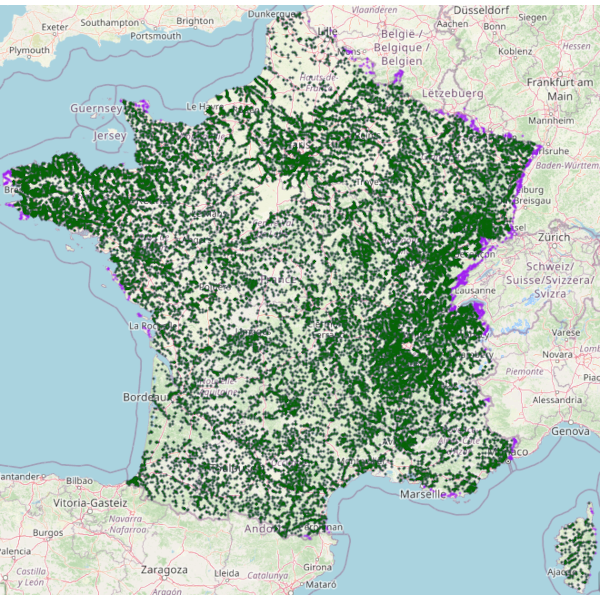
\includegraphics{images/stations_france_v2bis.png}
\caption{(\#fig:carte-france\_v2) Visualisation des stations ``récupérées'' par v2.}
\end{figure}

\newpage

La dernière étape est l'ajout de ces stations dans la base EDA.

\begin{Shaded}
\begin{Highlighting}[]
\NormalTok{station\_aspe\_france }\OtherTok{\textless{}{-}}\NormalTok{ station\_aspe\_france\_buff}

\CommentTok{\# Write station table in the database}
\NormalTok{DBI}\SpecialCharTok{::}\FunctionTok{dbExecute}\NormalTok{(con, }\StringTok{"DROP TABLE if exists france.station\_aspe;"}\NormalTok{)}
\NormalTok{DBI}\SpecialCharTok{::}\FunctionTok{dbWriteTable}\NormalTok{(con, }\StringTok{"station\_aspe"}\NormalTok{, station\_aspe\_france) }
\NormalTok{DBI}\SpecialCharTok{::}\FunctionTok{dbExecute}\NormalTok{(con, }\StringTok{"ALTER TABLE station\_aspe set schema france"}\NormalTok{)}
\end{Highlighting}
\end{Shaded}

\newpage

\hypertarget{ruxe9cupuxe9ration-des-points-de-pruxe9luxe8vements}{%
\subsection{Récupération des points de prélèvements}\label{ruxe9cupuxe9ration-des-points-de-pruxe9luxe8vements}}

\PageDerniere

\end{document}
